% !TeX program = xelatex
% Approved increment: textbook section 2.3, including its detailed models.
\documentclass[12pt,a4paper]{article}
\RequirePackage{array}[=2024-06-01]
% !TeX root = ../2/main.tex
\usepackage[a4paper,margin=25mm,headheight=16pt]{geometry}
\usepackage{amsmath,amssymb}
\usepackage{graphicx}
\usepackage{booktabs}
\usepackage{tabularx}
\usepackage{siunitx}
\usepackage{tikz}
\usepackage{circuitikz}
\usepackage[unicode,hidelinks]{hyperref}
\usepackage{xepersian}
% Only the regular B Nazanin file is installed; synthesize bold explicitly.
\settextfont[Path=C:/Windows/Fonts/,AutoFakeBold=2,AutoFakeSlant=0.2]{B-NAZANIN.TTF}
% B Nazanin lacks U+066A (Arabic percent), required by xepersian's digit setup.
% Arial covers the complete required digit/punctuation set; Persian prose remains B Nazanin.
\setdigitfont[Path=C:/Windows/Fonts/,BoldFont=arialbd.ttf,ItalicFont=ariali.ttf,BoldItalicFont=arialbi.ttf]{arial.ttf}
\setmathdigitfont[Path=C:/Windows/Fonts/,BoldFont=arialbd.ttf,ItalicFont=ariali.ttf,BoldItalicFont=arialbi.ttf]{arial.ttf}
\setlatintextfont{TeX Gyre Termes}
% B Nazanin does not contain the default itemize bullet and dash glyphs.
\renewcommand{\labelitemi}{\(\bullet\)}
\renewcommand{\labelitemii}{\(\circ\)}
\renewcommand{\labelitemiii}{\(\diamond\)}
\setlength{\parindent}{0pt}
\setlength{\parskip}{0.5em}
\linespread{1.25}
\newcommand{\exercise}[1]{\section*{تمرین #1}}
% !TeX root = ../2/main.tex
% Shared title page for every assignment.
% Change only \AssignmentNumber and \AssignmentDate in each main document.

\newcommand{\AssignmentNumber}[1]{\gdef\assignmentnumber{#1}}
\newcommand{\AssignmentDate}[1]{\gdef\assignmentdate{#1}}

\newcommand{\assignmentnumber}{---}
\newcommand{\assignmentdate}{---}

% Stable course metadata
\newcommand{\universityname}{دانشگاه صنعتی امیرکبیر}
\newcommand{\universityalias}{پلی‌تکنیک تهران}
\newcommand{\facultyname}{دانشکده مهندسی کامپیوتر}
\newcommand{\coursename}{طراحی مدارهای مجتمع پرتراکم پیشرفته}
\newcommand{\studentname}{محمد خلیلی اصل}
\newcommand{\instructorname}{دکتر مهدی صدیقی}

\newcommand{\MakeAssignmentCover}{%
  \begin{titlepage}
    \thispagestyle{empty}
    \centering
    \linespread{1}\selectfont

    \vspace*{0mm}
    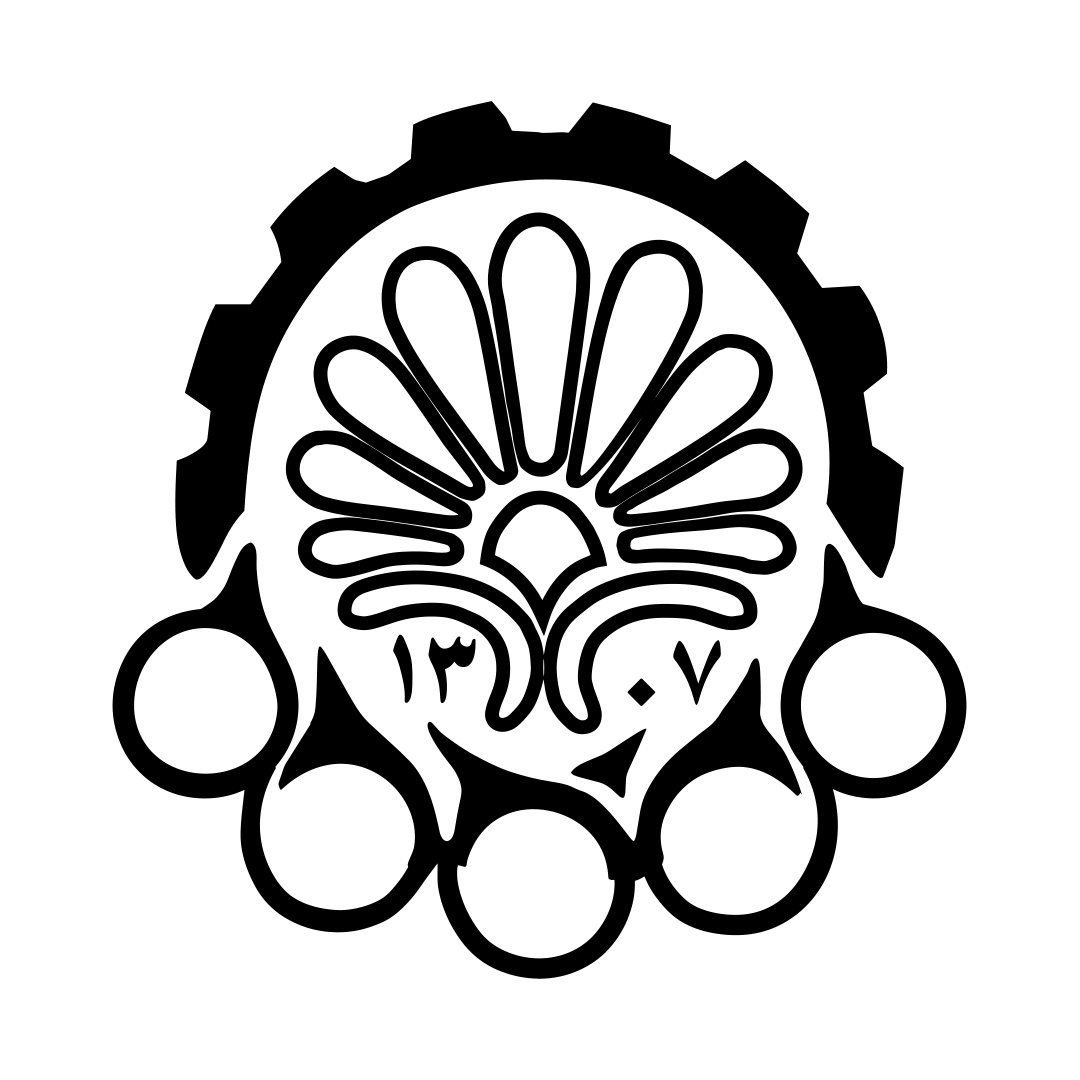
\includegraphics[width=44mm]{assets/aut-logo-black.png}\par
    \vspace{3mm}

    {\Large\bfseries \universityname\par}
    \vspace{1mm}
    {\large (\universityalias)\par}
    \vspace{1mm}
    {\large \facultyname\par}

    \vspace{8mm}
    {\Large\bfseries درس \coursename\par}

    \vspace{12mm}
    {\large عنوان\par}
    \vspace{2mm}
    {\LARGE\bfseries تمرین شماره \assignmentnumber\par}

    \vspace{10mm}
    {\large تهیه‌کننده\par}
    \vspace{2mm}
    {\Large\bfseries \studentname\par}

    \vspace{10mm}
    {\large استاد درس\par}
    \vspace{2mm}
    {\Large\bfseries \instructorname\par}

    \vspace{10mm}
    {\Large \assignmentdate\par}
    \vfill
  \end{titlepage}
  \setcounter{page}{1}%
}


\XeTeXgenerateactualtext=1
\newcommand{\secnum}[1]{\mbox{\beginL#1\endL}}
\setlength{\emergencystretch}{3em}
\widowpenalty=10000
\clubpenalty=10000
\AtBeginDocument{\DeclareSIPrefix{\micro}{\text{\lr{µ}}}{-6}}
\hypersetup{pdftitle={جزوه اول، مدل‌های MOS Capacitance و مشخصه C-V}}
\AssignmentNumber{جزوه اول، ظرفیت‌های \lr{MOS}}
\AssignmentDate{بخش \secnum{۲.۳} کتاب}
\patchcmd{\MakeAssignmentCover}{تمرین شماره \assignmentnumber}{\assignmentnumber}{}{\errmessage{Cover title replacement failed}}
\begin{document}
\MakeAssignmentCover
\section*{هدف و مسیر مطالعه}
در تحلیل جریان، رابطه بار کانال و ولتاژ \lr{Gate} را به کار بردیم.
اکنون تغییر بار پایانه‌ها را دنبال می‌کنیم تا بار ورودی گیت و ظرفیت‌های ناخواسته
خروجی را تخمین بزنیم. معنای مشتق و میانگین‌گیری در محل استفاده توضیح داده می‌شود.
با درنظرگرفتن نگذرانده‌بودن \lr{Digital Electronics}، مدل مدار معادل و شرایط
جمع‌کردن ظرفیت‌ها نیز با مثال معرفی می‌شوند.

دامنه این متن، بخش \secnum{۲.۳} کتاب در صفحات چاپی ۶۸ تا ۷۳ و اسلایدهای ۲۳ و ۲۴
مجموعه \lr{01} است \cite{weste,mos}. هر سه زیربخش مدل ساده، مدل تفصیلی
\lr{Gate} و مدل تفصیلی \lr{Diffusion} پوشش داده می‌شوند.
استخراج ضریب \(2/3\)، توضیح ظرفیت معادل بر پایه تغییر بار و تمرین‌های افزوده،
بسط آموزشی مدل‌های مرجع هستند. در شکل‌ها و مثال‌های افزوده، فرض‌های عددی مشخص می‌شوند.

نماد \(C_0=WLC_{\mathrm{ox}}\) ظرفیت هندسی اکسید روی کانال است.
\(C_{GS,i},C_{GD,i},C_{GB,i}\) مؤلفه‌های \lr{Intrinsic} مدل کتاب را نشان می‌دهند.
پسوند \(\mathrm{ov}\) سهم \lr{Overlap} و نماد بدون پسوند \(i\)، در مدار معادل
کامل این جزوه، مجموع سهم‌های همان دو پایانه را نشان می‌دهد.
این تفکیک مانع جمع‌کردن دوباره یک سهم در مدل‌های با دقت متفاوت می‌شود.

جدول‌ها و فرمول‌ها از مدل‌های آموزشی کتاب استفاده می‌کنند. برای کاربرد عددی در
فناوری واقعی، پارامترها و روش استخراج مدل همان فناوری لازم است.
\tableofcontents
\clearpage
\section{ظرفیت وابسته به ولتاژ و مدل ساده \lr{MOS}}
\subsection{معنای \lr{C-V} و تغییر بار}
ظرفیت بیان می‌کند که برای تغییر اختلاف ولتاژ دو رسانا، چه مقدار بار باید جابه‌جا
شود. برای خازن خطی با ظرفیت ثابت \(C\)، تغییر بار و اختلاف ولتاژ متناسب‌اند
\begin{equation}
 \Delta Q=C\Delta V.
 \label{eq:cv-linear-charge}
\end{equation}
در افزاره \lr{MOS}، وضعیت کانال و ضخامت ناحیه \lr{Depletion} با بایاس تغییر
می‌کنند. در نتیجه، ظرفیت نیز به ولتاژ وابسته است. نام \lr{C-V Characteristics}
همین وابستگی را بیان می‌کند \cite[آغاز بخش \secnum{۲.۳}]{weste}.

برای ظرفیت غیرخطی، شیب نمودار بار نسبت به ولتاژ در نقطه کار را تعریف می‌کنیم
\begin{equation}
 C(V)=\frac{dQ}{dV},\qquad dQ=C(V)\,dV.
 \label{eq:cv-differential}
\end{equation}
مشتق \(dQ/dV\) یعنی نسبت تغییر بسیار کوچک بار به تغییر بسیار کوچک ولتاژ.
واحد آن \unit{\coulomb\per\volt}، برابر \unit{\farad} است.
برای تغییر کوچک پیرامون \(V_0\)، رابطه
\(\Delta Q\approx C(V_0)\Delta V\) کاربرد دارد.
برای تغییر بزرگ، باید ظرفیت همه بخش‌های مسیر ولتاژ را در نظر گرفت.

اگر ولتاژ از \(V_1\) به \(V_2\) تغییر کند، جمع پیوسته تغییرهای بار می‌دهد
\begin{equation}
 \Delta Q=\int_{V_1}^{V_2}C(V)\,dV,\qquad
 C_{\mathrm{eff},Q}=\frac{\Delta Q}{V_2-V_1}
 =\frac1{V_2-V_1}\int_{V_1}^{V_2}C(V)\,dV.
 \label{eq:cv-charge-equivalent}
\end{equation}
\(C_{\mathrm{eff},Q}\) یک ظرفیت ثابت معادل از نظر بار جابه‌جاشده در همین بازه است.
این استخراج از تعریف ظرفیت است. کتاب برای تخمین دستی نیز از ظرفیت متوسط
طی گذار استفاده می‌کند. تغییر بازه یا حرکت هم‌زمان پایانه دیگر می‌تواند مقدار
معادل را تغییر دهد.

برای مثال فرضی \(C(V)=C_a(1-aV)\)، \(C_a=\qty{2}{\femto\farad}\)،
\(a=\qty{0.2}{\per\volt}\) و بازه صفر تا \qty{1}{\volt}، ظرفیت در ابتدا
\qty{2}{\femto\farad} و در انتها \qty{1.6}{\femto\farad} است.
با جمع مساحت زیر خط، میانگین \qty{1.8}{\femto\farad} و تغییر بار
\qty{1.8}{\femto\coulomb} می‌شود. چون در این مثال \(C(V)\) خطی است، میانگین
دو مقدار انتهایی با میانگین انتگرالی برابر است.
در رابطه غیرخطی، میانگین دو سر بازه یک تقریب است.

\subsection{مدار معادل پنج ظرفیت و پایانه مرجع}
کتاب در شکل \secnum{۲.۱۳} پنج ظرفیت عمده را نشان می‌دهد. سه سهم
\(C_{GS},C_{GD},C_{GB}\) به \lr{Gate}، و دو سهم \(C_{SB},C_{DB}\)
به پیوندهای \lr{Diffusion} و \lr{Body} مربوط‌اند.
شکل \ref{fig:cv-network} این ارتباط را بدون جزئیات ترانزیستور بازترسیم می‌کند.
این نمایش، مدل خازنی آموزشی بایاس‌شده است \cite[صفحه ۷۳]{weste}.
\begin{figure}[ht]
\centering
\begin{latin}
\begin{circuitikz}[font=\small]
\draw (0,3) node[circ] (G) {} node[above] {Gate};
\draw (-3,0) node[circ] (S) {} node[left] {Source};
\draw (3,0) node[circ] (D) {} node[right] {Drain};
\draw (0,-3) node[circ] (B) {} node[below] {Body};
\draw (G) to[C,l=$C_{GS}$] (S);
\draw (G) to[C,l_=$C_{GD}$] (D);
\draw (S) to[C,l=$C_{SB}$] (B);
\draw (D) to[C,l_=$C_{DB}$] (B);
\draw (G) to[C,l=$C_{GB}$] (B);
\end{circuitikz}
\end{latin}
\caption{ارتباط پایانه‌ای ظرفیت‌های اصلی در مدل آموزشی کتاب.
سهم‌های \lr{Intrinsic} و \lr{Overlap} در \(C_{GS}\) و \(C_{GD}\) جمع شده‌اند
\cite[شکل \secnum{۲.۱۳}]{weste}.}
\label{fig:cv-network}
\end{figure}

برای یک خازن ثابت میان گره \(A\) و گره \(B\)، بار سمت \(A\) برابر
\(Q_A=C(V_A-V_B)\) و جریان ورودی آن سمت برابر است با
\begin{equation}
 i_A=C\left(\frac{dV_A}{dt}-\frac{dV_B}{dt}\right).
 \label{eq:cv-two-terminal-current}
\end{equation}
اگر \(B\) ثابت بماند، \(dV_B/dt=0\) و ظرفیت مانند بار متصل به مرجع ثابت دیده
می‌شود. اتصال \lr{Body} به تغذیه ثابت نیز برای تحلیل تغییرات ولتاژ چنین نقشی دارد.
اگر هر دو گره حرکت کنند، اختلاف تغییرهای آن‌ها در جریان مؤثر است.

ظرفیت‌های متصل به یک گره را هنگامی مستقیم جمع می‌کنیم که سمت دیگرشان در تحلیل
مورد نظر مرجع ثابت باشد یا اثر حرکت آن جداگانه منظور شده باشد.
برای نمونه، ظرفیت \lr{Drain} به \lr{Body} ثابت، سهمی از بار خروجی است.
ظرفیت \lr{Gate} مرحله بعد، از دید خروجی مرحله قبل بار ورودی آن مرحله محسوب می‌شود.

\subsection{مدل صفحه‌ای \lr{Gate} و ظرفیت بر واحد عرض}
در مدل ساده بخش \secnum{۲.۳.۱}، ظرفیت \lr{Gate} روی کانال از رابطه
\begin{equation}
 C_g\approx C_0=WLC_{\mathrm{ox}},\qquad
 C_{\mathrm{ox}}=\frac{\varepsilon_{\mathrm{ox}}}{t_{\mathrm{ox}}}
 \label{eq:cv-simple-gate}
\end{equation}
تخمین زده می‌شود. \(C_{\mathrm{ox}}\) ظرفیت بر واحد سطح و \(C_g\) ظرفیت کل است.
کانال پایانه مستقل بیرونی ندارد. کتاب برای تخمین مقدماتی، صفحه پایین خازن را
به \lr{Source} نسبت می‌دهد و از \(C_{GS}\) استفاده می‌کند. در مدل تفصیلی،
این نسبت‌دادن به ناحیه کاری وابسته خواهد بود
\cite[رابطه \secnum{۲.۱۲} و اسلاید ۲۴]{weste,mos}.

در فناوری با طول ثابت، می‌توان \(L\) را در ضریب ظرفیت بر واحد عرض جذب کرد
\begin{equation}
 c_w=C_{\mathrm{ox}}L
 =\frac{\varepsilon_{\mathrm{ox}}L}{t_{\mathrm{ox}}},\qquad C_g\approx c_wW.
 \label{eq:cv-width-coefficient}
\end{equation}
نماد \(c_w\) همان \(C_{\mathrm{permicron}}\) در کتاب است، با واحد رایج
\unit{\femto\farad\per\micro\metre}.
اگر \(c_w=\qty{2}{\femto\farad\per\micro\metre}\) و
\(W=\qty{0.6}{\micro\metre}\) باشند، ظرفیت \(C_g\approx\qty{1.2}{\femto\farad}\)
می‌شود. واحد طول در ضرب حذف می‌شود.

از نظر تبدیل واحد، \(\qty{1}{\femto\farad\per\micro\metre}=10^{-9}\,
\unit{\farad\per\metre}\) است. برای نمونه فرضی،
\(C_{\mathrm{ox}}=\qty{4}{\femto\farad\per\micro\metre\squared}\) و
\(L=\qty{0.25}{\micro\metre}\) ضریب \(c_w=\qty{1}{\femto\farad\per\micro\metre}\)
می‌دهند. با \(W=\qty{2}{\micro\metre}\)، ظرفیت \qty{2}{\femto\farad} است.

اگر \(L\) و \(t_{\mathrm{ox}}\) با ضریب یکسان کوچک شوند و گذردهی ثابت بماند،
نسبت \(L/t_{\mathrm{ox}}\) و در نتیجه \(c_w\) ثابت می‌ماند.
اگر عرض نیز با همان ضریب کوچک شود، ظرفیت کل به نسبت عرض کاهش می‌یابد.
کتاب مقدار حدود \qty{2}{\femto\farad\per\micro\metre} را برای فرآیندهای
قدیمی‌تر و حدود \qty{1}{\femto\farad\per\micro\metre} را در نمونه‌های
\qty{90}{\nano\metre} و \qty{65}{\nano\metre} ذکر می‌کند.
این اعداد تخمین‌های تاریخی همان مرجع هستند \cite[روابط \secnum{۲.۱۳} و \secnum{۲.۱۴}]{weste}.

\subsection{مدل ساده \lr{Diffusion} و ارتباط با بار خروجی}
پیوند \lr{p-n} میان \lr{Source} یا \lr{Drain} و \lr{Body} در بایاس معکوس
ناحیه \lr{Depletion} دارد. دو ناحیه رسانا در دو سوی این ناحیه کم‌حامل، رفتار
خازنی ایجاد می‌کنند. پهنای ناحیه با ولتاژ تغییر می‌کند، بنابراین ظرفیت به بایاس
وابسته است \cite[اسلاید ۲۳ و صفحه ۶۹]{mos,weste}.
اصطلاح \lr{Diffusion Capacitance} در این فصل نام رایج طراحان مدار برای همین
ظرفیت پیوندی \lr{Depletion} است. این کاربرد در پانوشت صفحه ۶۹ توضیح داده شده است.

کتاب برای تخمین دستی، \(C_{SB}\) و \(C_{DB}\) ناحیه‌های دارای \lr{Contact}
را هم‌مرتبه ظرفیت \lr{Gate} می‌گیرد و در بسیاری از مثال‌ها ضریب حدود
\qty{1}{\femto\farad\per\micro\metre} به‌ازای عرض را به کار می‌برد.
ضریب مناسب هر فناوری و هندسه باید از داده همان مدل برداشته شود.
هندسه ناحیه مشترک و بدون \lr{Contact} در تحلیل دقیق اثر دارد
\cite[صفحه ۷۰]{weste}.

در مثال فرضی، یک \lr{Inverter} خروجیِ متصل به دو \lr{Inverter} مشابه بعدی دارد.
عرض‌ها \(W_n=\qty{1}{\micro\metre}\)، \(W_p=\qty{2}{\micro\metre}\) و
تمام ضریب‌های ساده \lr{Gate} و \lr{Drain} برابر
\qty{1}{\femto\farad\per\micro\metre} فرض می‌شوند. ظرفیت سیم
\qty{0.5}{\femto\farad} است. هر ورودی بعدی \qty{3}{\femto\farad} و مجموع
\lr{Drain}های خروجی راه‌انداز نیز \qty{3}{\femto\farad} می‌دهد. پس
\begin{equation}
 C_L\approx2(1+2)+(1+2)+0.5=\qty{9.5}{\femto\farad}.
 \label{eq:cv-load-example}
\end{equation}
اعداد داخل جمع، ظرفیت در واحد \unit{\femto\farad} هستند.
\lr{Source}های راه‌انداز به ریل ثابت متصل‌اند و در این مدل، سهم پیوندی مستقیم
خروجی از \lr{Drain}های آن می‌آید. با ولتاژ تغییر \qty{1}{\volt} و جریان متوسط
فرضی \qty{100}{\micro\ampere}، تخمین \(C_L\Delta V/I\) برابر
\qty{95}{\pico\second} می‌شود. این تخمین از ضریب‌های ساده و مرجع‌های ثابت استفاده می‌کند.

\subsection{تمرین‌های پاسخ‌دار مدل ساده}
\textbf{تمرین ۱.} اگر \(C_{\mathrm{ox}}=\qty{5}{\femto\farad\per\micro\metre\squared}\)،
\(L=\qty{0.2}{\micro\metre}\) و \(W=\qty{0.8}{\micro\metre}\) باشند،
ظرفیت چقدر است؟ ابتدا ضریب بر واحد عرض و سپس ظرفیت کل را می‌یابیم.
\[
 \begin{aligned}
 c_w&=5(0.2)=\qty{1}{\femto\farad\per\micro\metre},\\
 C_g&=1(0.8)=\qty{0.8}{\femto\farad}.
 \end{aligned}
\]

\textbf{تمرین ۲.} در مقیاس‌بندی ایدئال، \(L\)، \(W\) و ضخامت اکسید هر یک
نصف شوند. نسبت ظرفیت جدید به قبلی چیست؟ \(C_{\mathrm{ox}}\) دو برابر و
\(WL\) یک‌چهارم می‌شود، پس \(C_g\) نصف خواهد شد.
این نتیجه به فرض ثابت‌بودن گذردهی و مدل صفحه‌ای وابسته است.

\textbf{تمرین ۳.} سه ظرفیت \qty{2}{\femto\farad}، \qty{3}{\femto\farad} و
\qty{1}{\femto\farad} از یک گره به مرجع ثابت وصل‌اند. برای تغییر
\qty{0.8}{\volt}، بار جابه‌جاشده چقدر است؟ ظرفیت کل
\(2+3+1=\qty{6}{\femto\farad}\) و تغییر بار
\(6(0.8)=\qty{4.8}{\femto\coulomb}\) می‌شود.
\clearpage

\section{مدل تفصیلی ظرفیت \lr{Gate}}
\subsection{سهم \lr{Intrinsic} و وابستگی صفحه پایین به ناحیه کاری}
در مدل تفصیلی بخش \secnum{۲.۳.۲}، ظرفیت \lr{Gate} شامل سهم روی کانال و سهم
هم‌پوشانی با \lr{Source} و \lr{Drain} است. سهم روی کانال، \lr{Intrinsic}
نام دارد. ظرفیت هندسی مرجع را به صورت
\begin{equation}
 C_0=WLC_{\mathrm{ox}}
 \label{eq:cv-czero}
\end{equation}
تعریف می‌کنیم. این کمیت مرجع برای مقایسه ناحیه‌هاست. تقسیم ظرفیت میان پایانه‌ها
به محل بار پاسخ‌دهنده به \lr{Gate} بستگی دارد
\cite[صفحه ۷۰، شکل \secnum{۲.۹}]{weste}.

در \lr{Cutoff}، کانال \lr{Strong Inversion} وجود ندارد. تغییر بار \lr{Gate}
عمدتاً با تغییر بار \lr{Body} جبران می‌شود. سهم مربوط، \(C_{GB,i}\) است.
در \lr{Accumulation}، حامل‌های غالب نزدیک سطح‌اند و این ظرفیت تقریباً
\(C_0\) است. در \lr{Depletion}، ناحیه کم‌حامل مانند فاصله اضافی میان بارهای
پاسخ‌دهنده عمل می‌کند و ظرفیت مؤثر کاهش می‌یابد.

برای درک مدل سری، \(C_{\mathrm{dep}}\) را ظرفیت کل ناحیه \lr{Depletion}
زیر \lr{Gate} می‌نامیم. چون در دو بخش سری، بزرگی تغییر بار یکسان و تغییرهای
ولتاژ جمع‌شونده‌اند، داریم
\begin{equation}
 \frac1{C_{GB,i}}\approx\frac1{C_0}+\frac1{C_{\mathrm{dep}}}
 \quad\Longrightarrow\quad
 C_{GB,i}\approx\frac{C_0C_{\mathrm{dep}}}{C_0+C_{\mathrm{dep}}}.
 \label{eq:cv-depletion-series}
\end{equation}
این توضیح تکمیلی، کاهش ظرفیت نشان‌داده‌شده در شکل \secnum{۲.۹} کتاب را بیان
می‌کند. اگر هر دو ظرفیت سری برابر \qty{6}{\femto\farad} باشند، حاصل
\(36/12=\qty{3}{\femto\farad}\) است.
افزایش پهنای ناحیه کم‌حامل، ظرفیت آن را کم می‌کند و ظرفیت سری نیز کاهش می‌یابد.

در \lr{Linear} با \(V_{GS}>V_{tn}\) و \(V_{DS}\) نزدیک صفر، کانال به هر دو
\lr{Source} و \lr{Drain} متصل است. مدل تقریبی کتاب سهم را برابر تقسیم می‌کند
\begin{equation}
 C_{GS,i}\approx\frac{C_0}{2},\qquad
 C_{GD,i}\approx\frac{C_0}{2},\qquad C_{GB,i}\approx0.
 \label{eq:cv-linear-partition}
\end{equation}
با افزایش \(V_{DS}\) در همان ناحیه، بار کانال نزدیک \lr{Drain} کمتر می‌شود.
سهم منتسب به \lr{Source} افزایش و سهم منتسب به \lr{Drain} کاهش می‌یابد.
جدول ساده کتاب، مقادیر نزدیک \(V_{DS}=0\) را برای ناحیه \lr{Linear} نمایندگی می‌کند.

در \lr{Saturation}، انتهای کانال از \lr{Drain} جدا شده و در این تقریب،
\(C_{GD,i}\approx0\) و \(C_{GB,i}\approx0\) هستند. ظرفیت مؤثر ذاتی به
\lr{Source} نسبت داده می‌شود و مقدار آن
\begin{equation}
 C_{GS,i}\approx\frac23C_0
 \label{eq:cv-sat-cap}
\end{equation}
است \cite[صفحه ۷۰ و جدول \secnum{۲.۱}]{weste}.
در مدل پیوسته، تغییر مؤلفه‌ها با نزدیک‌شدن به مرز نرم است.
جدول قطعه‌ای، این تغییر را برای تخمین دستی خلاصه می‌کند.

\clearpage
\subsection{استخراج ضریب دوسوم از بار کانال}
برای فهم ضریب \(2/3\)، از مدل بار موضعی بخش \secnum{۲.۲} استفاده می‌کنیم.
در این مدل، \(x\) فاصله از \lr{Source} و \(V(x)\) ولتاژ محلی کانال نسبت به
\lr{Source} است. اضافه‌ولتاژ گیت را با شرط مثبت‌بودن آن تعریف می‌کنیم.
\[
 V_{GT}=V_{GS}-V_{tn},\qquad V_{GT}>0.
\]
بزرگی بار متحرک قطعه‌ای به طول \(dx\)
برابر \(WC_{\mathrm{ox}}[V_{GT}-V(x)]dx\) است.
رابطه جریان محلی با \lr{Mobility} و آستانه ثابت، پس از انتگرال از صفر تا \(x\)، می‌دهد
\begin{equation}
 I_{DS}x=\mu_nWC_{\mathrm{ox}}
 \left[V_{GT}V(x)-\frac{V(x)^2}{2}\right].
 \label{eq:cv-potential-profile}
\end{equation}
در اشباع بلندکانال، \(I_{DS}=\mu_nC_{\mathrm{ox}}(W/2L)V_{GT}^2\) است.
با جای‌گذاری و تقسیم دو طرف بر \(\mu_nWC_{\mathrm{ox}}V_{GT}^2/2\)، نتیجه می‌شود
\begin{equation}
 \frac{x}{L}=2\frac{V(x)}{V_{GT}}-
 \left(\frac{V(x)}{V_{GT}}\right)^2,
 \qquad
 1-\frac{x}{L}=\left(1-\frac{V(x)}{V_{GT}}\right)^2.
 \label{eq:cv-square-profile}
\end{equation}
چون \(0\le V(x)\le V_{GT}\)، ریشه نامنفی را می‌گیریم، پس
\begin{equation}
 V_{GT}-V(x)=V_{GT}\sqrt{1-\frac{x}{L}}.
 \label{eq:cv-root-profile}
\end{equation}
بار متحرک در نزدیکی \lr{Source} بیشینه و در انتهای مدل کانال صفر است.
جمع بار همه قطعه‌ها، با تغییر متغیر بی‌بعد \(u=x/L\)، می‌دهد
\begin{align}
 Q_{\mathrm{ch}}
 &=WC_{\mathrm{ox}}V_{GT}\int_0^L\sqrt{1-\frac{x}{L}}\,dx\notag\\
 &=WLC_{\mathrm{ox}}V_{GT}\int_0^1\sqrt{1-u}\,du
 =\frac23 C_0V_{GT}.
 \label{eq:cv-sat-charge}
\end{align}
انتگرال آخر مساحت زیر منحنی \(\sqrt{1-u}\) است. برای محاسبه مرحله‌ای،
پادمشتق آن \(-\tfrac23(1-u)^{3/2}\) است. مقدار در انتهای بازه صفر و در
ابتدای بازه \(-2/3\) می‌شود. تفاضل دو مقدار، \(2/3\) است.
عامل \(2/3\) از شکل توزیع بار در کانال حاصل می‌شود.

در این مدل، بخش متغیر بار \lr{Gate} با بزرگی بار کانال متناظر است.
با ثابت‌گرفتن آستانه و سایر بایاس‌های لازم در تقریب ذاتی، تغییر \(V_{GS}\)
همان تغییر \(V_{GT}\) است. بنابراین
\begin{equation}
 C_{GS,i}\approx\frac{dQ_G}{dV_{GS}}
 =\frac{d[(2/3)C_0(V_{GS}-V_{tn})]}{dV_{GS}}
 =\frac23 C_0.
 \label{eq:cv-sat-derivative}
\end{equation}
این استخراج تکمیلی، مقدار جدول کتاب را در فرض‌های ایدئال توضیح می‌دهد.
مدل دقیق‌تر مبتنی بر بار پایانه‌ها، تغییرات بار و جریان را با روش سازگار مدل
فناوری محاسبه می‌کند. کتاب در پایان این زیربخش به \lr{Charge-based Model} اشاره دارد.

\subsection{جدول ناحیه‌ها و تفسیر \lr{Cutoff}}
جدول \ref{tab:cv-intrinsic} مؤلفه‌های ذاتی را یکجا نشان می‌دهد.
مؤلفه‌های \lr{Overlap} در این جدول به صورت جداگانه در نظر گرفته خواهند شد.
\begin{table}[ht]
\centering
\caption{مدل تقریبی ظرفیت ذاتی، با روشن‌کردن شرط‌های جدول \secnum{۲.۱} کتاب.}
\label{tab:cv-intrinsic}
\begin{tabular}{cccc}
\toprule
کمیت & \lr{Cutoff} & \lr{Linear} با \(V_{DS}\approx0\) & \lr{Saturation}\\
\midrule
\(C_{GB,i}\) & \(\le C_0\) & \(0\) & \(0\)\\
\(C_{GS,i}\) & \(0\) & \(C_0/2\) & \(2C_0/3\)\\
\(C_{GD,i}\) & \(0\) & \(C_0/2\) & \(0\)\\
\(C_{gc}=C_{GB,i}+C_{GS,i}+C_{GD,i}\) & \(\le C_0\) & \(C_0\) & \(2C_0/3\)\\
\bottomrule
\end{tabular}
\end{table}
در سطر آخر جدول کتاب، برای \lr{Cutoff} مقدار ساده‌شده \(C_0\) آمده است،
درحالی‌که سطر \(C_{GB}\) و متن صفحه ۷۰، کاهش ظرفیت در \lr{Depletion} را بیان
می‌کنند. مقدار \(C_0\) با تقریب \lr{Accumulation} سازگار است.
در این جزوه، علامت \(\le\) در سطر مجموع حفظ شده تا وابستگی بایاس آشکار بماند.
کتاب هشدار می‌دهد که استفاده همیشگی از \(C_0\)، ظرفیت افزاره نزدیک زیر آستانه
را به‌طور قابل‌توجهی بیش‌برآورد می‌کند \cite[صفحه ۷۲]{weste}.

در \lr{Cutoff}، جریان هدایت کانال در مدل مرتبه اول صفر است، اما با تغییر
ولتاژ، بار \lr{Gate} و ناحیه‌های پیوندی می‌تواند تغییر کند.
به همین دلیل، مدار خاموش نیز در تحلیل گذرا ظرفیت دارد.

\subsection{\lr{Overlap}، \lr{Fringing} و ظرفیت کل}
در افزاره واقعی، \lr{Gate} بخشی از ناحیه‌های \lr{Source} و \lr{Drain} را
می‌پوشاند و میدان‌های لبه‌ای، یا \lr{Fringing Fields}، نیز روی آن‌ها ختم می‌شوند.
این سهم‌ها در مدل کتاب به ظرفیت‌های \lr{Overlap} افزوده می‌شوند.
ضریب بر واحد عرض آن‌ها را \(c_{GS,\mathrm{ov}}\) و
\(c_{GD,\mathrm{ov}}\) می‌نامیم. این دو نماد متناظر با ضرایب
\(C_{gsol}\) و \(C_{gdol}\) در رابطه \secnum{۲.۱۵} کتاب هستند.
ظرفیت کل هر سهم چنین است
\begin{equation}
 C_{GS,\mathrm{ov}}=c_{GS,\mathrm{ov}}W,\qquad
 C_{GD,\mathrm{ov}}=c_{GD,\mathrm{ov}}W.
 \label{eq:cv-overlap}
\end{equation}
کتاب مقادیر معمول آن مثال‌ها را حدود \num{0.2} تا
\qty{0.4}{\femto\farad\per\micro\metre} بیان می‌کند
\cite[صفحه ۷۱، شکل \secnum{۲.۱۰}]{weste}.
در مدل ضرایب ثابت این بخش، سهم \lr{Overlap} با عرض رشد می‌کند.

با قرارداد این جزوه، جمع سهم ذاتی و هم‌پوشانی به صورت زیر است
\begin{equation}
 C_{GS}=C_{GS,i}+C_{GS,\mathrm{ov}},\qquad
 C_{GD}=C_{GD,i}+C_{GD,\mathrm{ov}},\qquad
 C_{GB}\approx C_{GB,i}.
 \label{eq:cv-total-components}
\end{equation}
در اشباع، \(C_{GD,i}\) در جدول ایدئال صفر است و \(C_{GD}\) می‌تواند سهم
\lr{Overlap} داشته باشد. اگر برای هر دو سمت ضریب یکسان \(c_{\mathrm{ov}}\)
به کار رود، تقریب کلی کتاب برای تخمین تأخیر
\(C_g\approx C_0+2c_{\mathrm{ov}}W\) است.
برای تحلیل ناحیه‌ای با پایانه‌های ثابت، سهم ذاتی همان ناحیه جایگزین \(C_0\) می‌شود.

مثال فرضی \(C_0=\qty{6}{\femto\farad}\)، \(W=\qty{2}{\micro\metre}\)
و \(c_{\mathrm{ov}}=\qty{0.3}{\femto\farad\per\micro\metre}\) را در نظر بگیرید.
هر سهم \lr{Overlap} برابر \qty{0.6}{\femto\farad} می‌شود.
در \lr{Linear} کم‌ولتاژ، دو ظرفیت برابرند.
\[
 C_{GS}=C_{GD}=3+0.6=\qty{3.6}{\femto\farad}.
\]
مجموع ظرفیت‌ها \qty{7.2}{\femto\farad} است. در اشباع، داریم
\[
 C_{GS}=4+0.6=\qty{4.6}{\femto\farad},\qquad
 C_{GD}=\qty{0.6}{\femto\farad}.
\]
مجموع ظرفیت‌های این حالت \qty{5.2}{\femto\farad} است.
در \lr{Accumulation}، مجموع تقریباً \(6+1.2=\qty{7.2}{\femto\farad}\) می‌شود.
در \lr{Depletion} فرضی با \(C_{\mathrm{dep}}=\qty{3}{\femto\farad}\)،
ظرفیت ذاتی از مدل سری به دست می‌آید.
\[
 C_{GB,i}=\frac{6(3)}{6+3}=\qty{2}{\femto\farad}.
\]
پس مجموع ظرفیت‌ها \qty{3.2}{\femto\farad} است.

\subsection{حرکت \lr{Source} و \lr{Drain} و ظرفیت مؤثر ورودی}
برای یک سهم ثابت \(C_{GX}\) میان \lr{Gate} و پایانه \(X\)، تغییر بار
\lr{Gate} برابر است با
\begin{equation}
 \Delta Q_G=C_{GX}(\Delta V_G-\Delta V_X).
 \label{eq:cv-moving-terminal}
\end{equation}
اگر \(\Delta V_G\ne0\)، با تقسیم بر تغییر ولتاژ ورودی، سهم مؤثر آن به دست می‌آید
\begin{equation}
 C_{\mathrm{eff},G}=C_{GX}\left(1-\frac{\Delta V_X}{\Delta V_G}\right).
 \label{eq:cv-miller-simple}
\end{equation}
در مدل خازن ثابت، برای پایانه ثابت، ضریب یک است.
اگر دو پایانه به یک اندازه و هم‌جهت حرکت کنند، اختلاف ولتاژ خازن تغییر نمی‌کند
و سهم جابه‌جایی بار آن در این گذار صفر است.
اگر هم‌اندازه و خلاف‌جهت حرکت کنند، ضریب دو می‌شود.
این تحلیل ساده، منشأ اثر حرکت پایانه دوم را نشان می‌دهد.

برای مثال، خازن \qty{1}{\femto\farad} میان دو گره را در نظر بگیرید.
\lr{Gate} از صفر به \qty{1}{\volt} می‌رود. اگر گره دیگر صفر بماند، تغییر بار
\qty{1}{\femto\coulomb} است. اگر گره دیگر از \qty{1}{\volt} به صفر برود،
تغییر اختلاف ولتاژ \qty{2}{\volt} و تغییر بار \qty{2}{\femto\coulomb} است.
اگر گره دیگر نیز از صفر به \qty{1}{\volt} برود، تغییر بار همین خازن صفر می‌شود.

کتاب در شکل \secnum{۲.۱۱} هفت ترکیب حرکت \lr{Source} و \lr{Drain} را برای
یک فرآیند \qty{0.35}{\micro\metre} گزارش می‌کند.
جدول \ref{tab:cv-data-dependent} داده‌های آن شکل را بازنویسی می‌کند.
در همه حالت‌ها، \lr{Gate} از صفر به یک می‌رود و \(C_g/C_0\) نسبت مؤثر گزارش‌شده
همان شکل است. این اعداد به افزاره و مسیر گذار مورد بررسی وابسته‌اند.
\begin{table}[ht]
\centering
\caption{وابستگی ظرفیت مؤثر \lr{Gate} به حرکت پایانه‌ها در شکل
\secnum{۲.۱۱} کتاب. پیکان، جهت گذار و عدد، مقدار منطقی ثابت را نشان می‌دهد \cite{weste}.}
\label{tab:cv-data-dependent}
\begin{tabular}{cccc}
\toprule
حالت شکل کتاب & \lr{Drain} & \lr{Source} & \(C_g/C_0\)\\
\midrule
۱ & \(\downarrow\) & \(\downarrow\) & \(1.3\)\\
۲ & \(\downarrow\) & \(0\) & \(1.1\)\\
۳ & \(0\) & \(0\) & \(1.0\)\\
۴ & \(1\) & \(0\) & \(0.80\)\\
۵ & \(1\) & \(1\) & \(0.42\)\\
۶ & \(1\) & \(\uparrow\) & \(0.31\)\\
۷ & \(\uparrow\) & \(\uparrow\) & \(0.13\)\\
\bottomrule
\end{tabular}
\end{table}
در ترانزیستور، مؤلفه‌های ظرفیت طی گذار نیز تغییر می‌کنند.
برای محاسبه دقیق‌تر باید بار پایانه‌ها در مسیر واقعی بایاس محاسبه شود.
مثال خازن ثابت، وابستگی به جهت حرکت را توضیح می‌دهد و اعداد جدول از مدل افزاره
و گذارِ منبع آمده‌اند. کتاب برای تخمین تأخیر، استفاده از ظرفیت مؤثر استخراج‌شده
از شبیه‌سازی را نیز مطرح می‌کند \cite[صفحات ۷۱ و ۷۲]{weste}.

\subsection{تمرین‌های پاسخ‌دار \lr{Gate Capacitance}}
\textbf{تمرین ۴.} برای \(C_0=\qty{9}{\femto\farad}\)، مؤلفه‌های ذاتی در
\lr{Linear} با \(V_{DS}\approx0\) و در اشباع چیست؟ در حالت اول،
\(C_{GS,i}=C_{GD,i}=\qty{4.5}{\femto\farad}\) و \(C_{GB,i}=0\) است.
در اشباع، \(C_{GS,i}=\qty{6}{\femto\farad}\) و دو سهم دیگر صفرند.

\textbf{تمرین ۵.} در تمرین قبل، \(W=\qty{3}{\micro\metre}\) و ضریب هر
\lr{Overlap} برابر \qty{0.2}{\femto\farad\per\micro\metre} باشد.
در اشباع، ظرفیت‌های کل و مجموعشان چقدر است؟ هر هم‌پوشانی
\qty{0.6}{\femto\farad} است. پس \(C_{GS}=\qty{6.6}{\femto\farad}\)،
\(C_{GD}=\qty{0.6}{\femto\farad}\) و مجموع \qty{7.2}{\femto\farad} می‌شود.

\textbf{تمرین ۶.} خازن ثابت \qty{2}{\femto\farad} به \lr{Gate} با تغییر
\qty{1}{\volt} متصل است. پایانه دیگر \qty{0.25}{\volt} هم‌جهت تغییر می‌کند.
ظرفیت مؤثر از دید \lr{Gate} چیست؟ از \eqref{eq:cv-miller-simple}، مقدار
\(2(1-0.25)=\qty{1.5}{\femto\farad}\) و تغییر بار
\qty{1.5}{\femto\coulomb} می‌شود.

\textbf{تمرین ۷.} در مدل سری \lr{Depletion}، \(C_0=\qty{8}{\femto\farad}\)
و \(C_{\mathrm{dep}}=\qty{8}{\femto\farad}\) باشد. اگر ظرفیت دوم نصف شود،
\(C_{GB,i}\) چه تغییری می‌کند؟ ابتدا \(64/16=\qty{4}{\femto\farad}\) است.
پس از تغییر، \(8(4)/(8+4)\approx\qty{2.67}{\femto\farad}\) می‌شود.
\clearpage

\section{مدل تفصیلی ظرفیت \lr{Diffusion}}
\subsection{مساحت کف و محیط کناره‌ها}
در بخش \secnum{۲.۳.۳} کتاب، ظرفیت پیوند \lr{Source} و \lr{Body} از دو سهم
کف و کناره محاسبه می‌شود. برای ناحیه مستطیلی با عرض \(W\) و امتداد بیرون
کانال \(D_{\mathrm{diff}}\)، مساحت و محیط برابرند با
\begin{equation}
 A=WD_{\mathrm{diff}},\qquad P=2W+2D_{\mathrm{diff}}.
 \label{eq:cv-diffusion-geometry}
\end{equation}
کتاب برای امتداد هندسی نماد \(D\) را به کار می‌برد. در این جزوه، پسوند
\(\mathrm{diff}\) آن را از نام پایانه \lr{Drain} مشخص می‌کند.
برای یک لبه مجاور کانال، طول لبه روبه‌روی \lr{Gate} برابر \(P_g=W\) و طول
باقی کناره‌ها \(P_{\mathrm{non}}=W+2D_{\mathrm{diff}}\) است.
جمع این دو، محیط کل \(P\) می‌شود \cite[شکل \secnum{۲.۱۲}]{weste}.

در مدل دوضریبی رابطه \secnum{۲.۱۶} کتاب، برای \lr{Source} داریم
\begin{equation}
 C_{SB}=A_SC_{jbs}+P_SC_{jbssw}.
 \label{eq:cv-two-coeff-junction}
\end{equation}
\(A_S\) و \(P_S\) به‌ترتیب مساحت و محیط \lr{Source} هستند.
\(C_{jbs}\) ظرفیت بر واحد سطح کف با واحدی مانند
\unit{\femto\farad\per\micro\metre\squared} و \(C_{jbssw}\) ظرفیت بر واحد طول
کناره با واحدی مانند \unit{\femto\farad\per\micro\metre} است.
هر دو حاصل‌ضرب واحد \unit{\femto\farad} دارند.

در مدل دارای ضریب مستقل برای لبه روبه‌روی کانال، جمع به صورت
\begin{equation}
 C_{SB}(V_R)=A_SC_A(V_R)+P_{\mathrm{non},S}c_{\mathrm{sw}}(V_R)
 +P_{g,S}c_{\mathrm{swg}}(V_R)
 \label{eq:cv-three-coeff-junction}
\end{equation}
نوشته می‌شود. \(C_A\) ضریب سطحی و \(c_{\mathrm{sw}},c_{\mathrm{swg}}\)
ضرایب طولی دو نوع کناره هستند. حروف کوچک در ضرایب طولی، واحد متفاوت را
در این جزوه روشن می‌کنند. همه طول‌های محیط میان دو دسته تقسیم شده‌اند.

کتاب در توضیح فناوری دارای \lr{Shallow Trench Isolation} یا \lr{STI}،
اهمیت متفاوت کناره عایق‌شده و کناره روبه‌روی کانال را توضیح می‌دهد
\cite[صفحه ۷۲]{weste}. برای \lr{Drain} نیز همین ساختار با مساحت \(A_D\)،
محیط‌های مربوط و ولتاژ پیوند \lr{Drain}-\lr{Body} به کار می‌رود.
پارامترهای \lr{nMOS} و \lr{pMOS} از فناوری همان افزاره گرفته می‌شوند.

\subsection{وابستگی به بایاس و معنای توان منفی}
\(V_R\ge0\) را بزرگی بایاس معکوس پیوند می‌نامیم. برای \lr{nMOS}، در سمت
\lr{Source}، \(V_R=V_S-V_B\) و در سمت \lr{Drain}، \(V_R=V_D-V_B\) است.
برای \lr{pMOS} با \lr{Body} پرپتانسیل‌تر، این بزرگی‌ها به‌ترتیب
\(V_B-V_S\) و \(V_B-V_D\) هستند. استفاده از بزرگی معکوس، دامنه ولتاژ فرمول
را برای هر دو نوع افزاره روشن می‌کند.

با افزایش بایاس معکوس، ناحیه \lr{Depletion} پهن‌تر می‌شود و ظرفیت کاهش می‌یابد.
رابطه سطحی کتاب چنین است
\begin{equation}
 C_A(V_R)=C_J\left(1+\frac{V_R}{\psi_0}\right)^{-M_J}
 =\frac{C_J}{(1+V_R/\psi_0)^{M_J}}.
 \label{eq:cv-area-bias}
\end{equation}
\(C_J\) ضریب سطحی در بایاس صفر، \(\psi_0\) پتانسیل داخلی پیوند و \(M_J\)
ضریب \lr{Junction Grading} است. کتاب برای \(M_J\) حدود \num{0.33} تا
\num{0.5} ذکر می‌کند \cite[رابطه \secnum{۲.۱۷}]{weste}.
داخل پرانتز بی‌بعد است، زیرا دو ولتاژ بر هم تقسیم شده‌اند.
توان منفی یعنی معکوس توان مثبت. اگر \(V_R\) افزایش یابد، مخرج برای \(M_J>0\)
بزرگ‌تر و ظرفیت کوچک‌تر می‌شود. در \(V_R=0\)، ضریب ظرفیت دقیقاً \(C_J\) است.

دو نوع ضریب کناره نیز با پارامترهای خود از روابط مشابه به دست می‌آیند
\begin{align}
 c_{\mathrm{sw}}(V_R)
 &=C_{JSW}\left(1+\frac{V_R}{\psi_{SW}}\right)^{-M_{JSW}},\notag\\
 c_{\mathrm{swg}}(V_R)
 &=C_{JSWG}\left(1+\frac{V_R}{\psi_{SWG}}\right)^{-M_{JSWG}}.
 \label{eq:cv-sidewall-bias}
\end{align}
در چاپ رابطه \secnum{۲.۲۰} کتاب، ضریب جلوی جمله سمت کانال با نماد
\(C_{JSW}\) دیده می‌شود، اما مثال \secnum{۲.۲} برای این سمت، پارامتر مستقل
\(C_{JSWG}\) می‌دهد. در \eqref{eq:cv-sidewall-bias} نام مستقل مطابق همان
مثال حفظ شده است. مدل انتخاب‌شده باید برای هر لبه ضریب مشخص داشته باشد.

این روابط برای بایاس معکوس یا صفر در نظر گرفته شده‌اند.
در بایاس مستقیم، مدل پیوند و هدایت آن به تحلیل مناسب آن شرایط نیاز دارد.
مثلاً جای‌گذاری بدون توجه به علامت بایاس \lr{pMOS} می‌تواند پایه توان کسری
را از دامنه معتبر مدل خارج کند.

\subsection{\lr{Thermal Voltage}، پتانسیل داخلی و لگاریتم طبیعی}
کتاب پتانسیل داخلی پیوند را به \lr{Doping} و دما مرتبط می‌کند
\begin{equation}
 \psi_0=v_T\ln\left(\frac{N_AN_D}{n_i^2}\right),\qquad
 v_T=\frac{kT}{q}.
 \label{eq:cv-built-in}
\end{equation}
\(N_A\) و \(N_D\) غلظت \lr{Acceptor} و \lr{Donor}، و \(n_i\) غلظت
حامل ذاتی‌اند. هر سه باید با واحد یکسان، مانند \unit{\per\centi\metre\cubed}،
جای‌گذاری شوند تا نسبت داخل لگاریتم بی‌بعد شود.
\(v_T\) در این رابطه \lr{Thermal Voltage} است.
\lr{Threshold Voltage} ترانزیستور در بخش‌های پیشین با \(V_{tn}\) یا
\(V_{tp}\) مشخص شده است \cite[رابطه \secnum{۲.۱۸}]{weste}.

\(T\) دمای مطلق بر حسب \unit{\kelvin}، \(k\) ثابت \lr{Boltzmann} و \(q\)
بزرگی بار الکترون است. با ثابت‌های گرد‌شده کتاب در \(T=\qty{300}{\kelvin}\)، داریم
\begin{equation*}
 v_T=\frac{(1.380\times10^{-23})(300)}{1.602\times10^{-19}}
 \,\unit{\volt}\approx\qty{0.02584}{\volt}\approx\qty{26}{\milli\volt}.
\end{equation*}
واحد \(kT\) انرژی و واحد \(q\) بار است. نسبت انرژی به بار، ولتاژ می‌شود.
برای تبدیل دمای سلسیوس، \(T\) بر حسب کلوین از افزودن \num{273.15} به مقدار
سلسیوس به دست می‌آید. مقدار \qty{300}{\kelvin} تقریب دمای اتاق در داده کتاب است.

\(\ln\) لگاریتم طبیعی با پایه \(e\approx\num{2.718}\) است.
اگر \(y=\ln x\)، آنگاه \(e^y=x\). برای محاسبه دستی می‌توان از
\(\ln(ab)=\ln a+\ln b\) و \(\ln(10^n)=n\ln10\) استفاده کرد.
برای غلظت‌های فرضی \(N_A=10^{16}\)، \(N_D=10^{17}\) و مقدار کتاب
\(n_i=1.45\times10^{10}\)، همگی در \unit{\per\centi\metre\cubed}، داریم
\begin{align*}
 \frac{N_AN_D}{n_i^2}
 &=\frac{10^{33}}{(1.45)^2\times10^{20}}
 \approx4.756\times10^{12},\\
 \ln(4.756\times10^{12})&=\ln4.756+12\ln10\approx29.19,\\
 \psi_0&\approx(0.02584)(29.19)\,\unit{\volt}\approx\qty{0.754}{\volt}.
\end{align*}
غلظت‌های فرضی این محاسبه برای توضیح لگاریتم انتخاب شده‌اند.
در مثال کتاب، مقدار \(\psi_0\) مستقیماً داده شده و همان مقدار استفاده می‌شود.

\subsection{حل مرحله‌ای مثال \texorpdfstring{\secnum{۲.۲}}{۲.۲} کتاب}
مثال \secnum{۲.۲}، ظرفیت \lr{Drain} یک \lr{nMOS} دارای \lr{Contact} را
در فناوری \qty{65}{\nano\metre} می‌خواهد. اندازه \(\lambda\)، عرض و امتداد
ناحیه به صورت زیر داده شده‌اند.
\[
 \lambda=\qty{25}{\nano\metre},\qquad
 W=4\lambda=\qty{0.1}{\micro\metre},\qquad
 D_{\mathrm{diff}}=5\lambda=\qty{0.125}{\micro\metre}.
\]
\lr{Body} به زمین وصل است و \(V_D\) ابتدا صفر و سپس \qty{1}{\volt} می‌شود
\cite[صفحه ۷۳]{weste}.
پارامترهای مثال چنین‌اند
\begin{align*}
 C_J&=\qty{1.2}{\femto\farad\per\micro\metre\squared},
 &M_J&=0.33,\\
 C_{JSW}&=\qty{0.1}{\femto\farad\per\micro\metre},
 &C_{JSWG}&=\qty{0.36}{\femto\farad\per\micro\metre},\\
 M_{JSW}&=M_{JSWG}=0.10,
 &\psi_0&=\qty{0.7}{\volt}.
\end{align*}
محاسبه کتاب برای کناره‌ها نیز از همین پتانسیل \qty{0.7}{\volt} استفاده می‌کند.
برای تطبیق آن، \(\psi_{SW}=\psi_{SWG}=\psi_0\) می‌گیریم.
هندسه ابتدا به صورت مستقل محاسبه می‌شود
\begin{align}
 A_D&=(0.1)(0.125)=\qty{0.0125}{\micro\metre\squared},\notag\\
 P_D&=2(0.1)+2(0.125)=\qty{0.45}{\micro\metre},\notag\\
 P_g&=W=\qty{0.1}{\micro\metre},\qquad
 P_{\mathrm{non}}=P_D-P_g=\qty{0.35}{\micro\metre}.
 \label{eq:cv-book-geometry}
\end{align}
در بایاس صفر، هر عامل \((1+V_R/\psi)^{-M}\) برابر یک است. با ضرب جداگانه هر
ضریب در هندسه متناظر، ظرفیت می‌شود
\begin{align*}
 C_{DB}(0)
 &=(0.0125)(1.2)+(0.35)(0.1)+(0.1)(0.36)\quad\unit{\femto\farad}\\
 &=(0.015+0.035+0.036)\,\unit{\femto\farad}
 =\qty{0.086}{\femto\farad}.
\end{align*}
در خط اول، واحد طول یا مساحت هر عدد هندسی، همان واحد داده‌شده در
\eqref{eq:cv-book-geometry} است و در ضرب با ضریب مناسب حذف می‌شود.
مجموع دو سهم کناره در این مثال \qty{0.071}{\femto\farad} است.

در \(V_D=\qty{1}{\volt}\)، بایاس معکوس \(V_R=\qty{1}{\volt}\) می‌شود.
عامل مشترک داخل پرانتز را \(r=1+1/0.7\approx2.42857\) می‌نامیم.
سهم کف در \(r^{-0.33}\) و سهم کناره‌ها در \(r^{-0.10}\) ضرب می‌شود، پس
\begin{align*}
 C_{DB}(1)
 &=0.015r^{-0.33}+0.071r^{-0.10}\quad\unit{\femto\farad}\\
 &\approx\qty{0.0762}{\femto\farad}\approx\qty{0.076}{\femto\farad}.
\end{align*}
برای محاسبه با ماشین‌حساب، ابتدا \(r\)، سپس \(r^{0.33}\) و \(r^{0.10}\)
را می‌یابیم و هر ضریب را بر توان مثبت مربوط تقسیم می‌کنیم.
کاهش ظرفیت با افزایش بایاس معکوس، با تفسیر پهن‌شدن \lr{Depletion} سازگار است.

کتاب برای تخمین دستی میانگین دو سر گذار را استفاده می‌کند
\begin{equation*}
 C_{DB,\mathrm{ends}}\approx\frac{0.086+0.076}{2}
 =\qty{0.081}{\femto\farad}.
\end{equation*}
این عدد، بازتولید تقریب مثال مرجع است. برای مقایسه، می‌توان معادل دقیق‌تر از
نظر بار همین تابع غیرخطی را با \eqref{eq:cv-charge-equivalent} محاسبه کرد.
برای هر مؤلفه \(C_a(1+V/\psi)^{-M}\) با \(M\ne1\)، انتگرال از صفر تا
\(V_{DD}\) به صورت
\begin{equation}
 \Delta Q=C_a\frac{\psi}{1-M}
 \left[\left(1+\frac{V_{DD}}{\psi}\right)^{1-M}-1\right]
 \label{eq:cv-junction-integral}
\end{equation}
درمی‌آید. عامل \(\psi\) از تبدیل متغیر \(u=1+V/\psi\) و
\(dV=\psi\,du\) حاصل می‌شود. با انتگرال توان \(u^{-M}\)، توان جدید
\(1-M\) و ضریب تقسیم بر \(1-M\) به دست می‌آیند.
جمع این رابطه برای سهم کف و دو کناره، سپس تقسیم بر \qty{1}{\volt}، ظرفیت
معادل بر پایه تغییر بار را می‌دهد. برای مقایسه عددی، با نگه‌داشتن ارقام میانی،
\(C_{\mathrm{eff},Q}\approx\qty{0.08023}{\femto\farad}\) و میانگین دو سر
گردنشده \(C_{\mathrm{ends}}\approx\qty{0.08108}{\femto\farad}\) می‌شود.
میانگین دو سر در این مثال حدود \num{1.1} درصد بیشتر است.
این محاسبه تکمیلی، دقت تقریب دستی را برای همین تابع و بازه می‌سنجد.

\subsection{هندسه \lr{Isolated}، \lr{Shared} و \lr{Merged}}
شکل \secnum{۲.۸} کتاب سه شکل اتصال دو ترانزیستور سری را نشان می‌دهد.
در \lr{Isolated Diffusion}، هر ترانزیستور ناحیه دارای \lr{Contact} خود را دارد
و دو ناحیه با سیم به هم وصل می‌شوند. در \lr{Shared Diffusion}، یک ناحیه مشترک
دارای \lr{Contact} میان دو \lr{Gate} قرار می‌گیرد.
در \lr{Merged Diffusion}، همان اتصال داخلی با ناحیه پیوسته بدون \lr{Contact}
ساخته می‌شود. شکل \ref{fig:cv-layout-types} فقط ناحیه داخلی مرتبط را نشان می‌دهد.

\begin{figure}[ht]
\centering
\begin{latin}
\PersianMathDigits
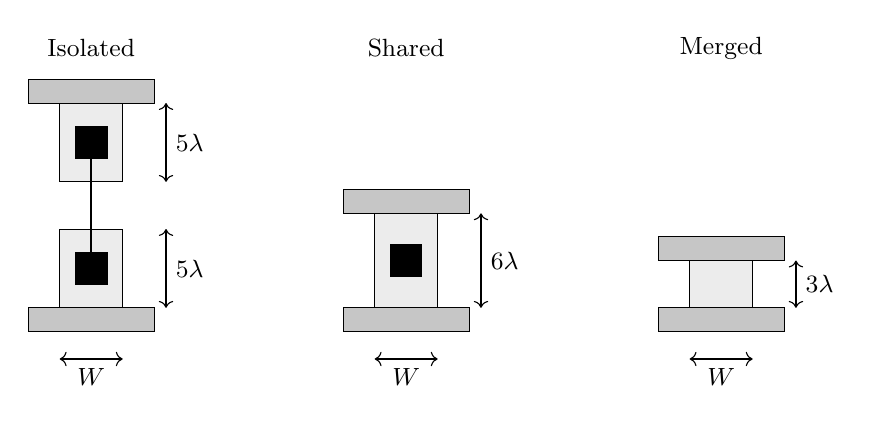
\begin{tikzpicture}[x=1cm,y=1cm,font=\small]
\node at (1,3.3) {Isolated};
\draw[fill=gray!15] (0.6,0) rectangle (1.4,1);
\draw[fill=gray!15] (0.6,1.6) rectangle (1.4,2.6);
\draw[fill=black] (0.8,0.3) rectangle (1.2,0.7);
\draw[fill=black] (0.8,1.9) rectangle (1.2,2.3);
\draw[thick] (1,0.5)--(1,2.1);
\draw[fill=gray!45] (0.2,-0.3) rectangle (1.8,0);
\draw[fill=gray!45] (0.2,2.6) rectangle (1.8,2.9);
\draw[<->] (1.95,0)--(1.95,1) node[midway,right] {$5\lambda$};
\draw[<->] (1.95,1.6)--(1.95,2.6) node[midway,right] {$5\lambda$};
\node at (5,3.3) {Shared};
\draw[fill=gray!15] (4.6,0) rectangle (5.4,1.2);
\draw[fill=black] (4.8,0.4) rectangle (5.2,0.8);
\draw[fill=gray!45] (4.2,-0.3) rectangle (5.8,0);
\draw[fill=gray!45] (4.2,1.2) rectangle (5.8,1.5);
\draw[<->] (5.95,0)--(5.95,1.2) node[midway,right] {$6\lambda$};
\node at (9,3.3) {Merged};
\draw[fill=gray!15] (8.6,0) rectangle (9.4,0.6);
\draw[fill=gray!45] (8.2,-0.3) rectangle (9.8,0);
\draw[fill=gray!45] (8.2,0.6) rectangle (9.8,0.9);
\draw[<->] (9.95,0)--(9.95,0.6) node[midway,right] {$3\lambda$};
\foreach \x in {1,5,9}{
 \draw[<->] (\x-0.4,-0.65)--(\x+0.4,-0.65) node[midway,below] {$W$};
}
\end{tikzpicture}
\end{latin}
\caption{بازترسیم آموزشی ناحیه داخلی دو ترانزیستور سری با هندسه شکل
\secnum{۲.۸} کتاب. نوارهای پهن تیره \lr{Gate}، مربع‌های سیاه \lr{Contact}
و مستطیل روشن \lr{Diffusion} است. خط میان دو \lr{Contact} حالت اول، اتصال
سیمی را نشان می‌دهد \cite{weste}.}
\label{fig:cv-layout-types}
\end{figure}

با \(W=4\lambda\)، \(\lambda=\qty{0.025}{\micro\metre}\) و پارامترهای
بایاس صفر مثال کتاب، می‌توان سهم پیوندی اتصال داخلی را مقایسه کرد.
برای دو ناحیه جدا، مساحت‌ها و کناره‌ها جمع می‌شوند. برای ناحیه مشترک یا
ادغام‌شده میان دو \lr{Gate}، دو لبه روبه‌روی کانال داریم، پس \(P_g=2W\)
و \(P_{\mathrm{non}}=2D_{\mathrm{diff}}\) می‌شود.
نتایج در جدول \ref{tab:cv-layout-area} آمده‌اند.

\begin{table}[ht]
\centering
\caption{مقایسه محاسبه‌شده فقط برای ظرفیت پیوندی گره داخلی در هندسه آموزشی شکل
\ref{fig:cv-layout-types} و بایاس صفر.}
\label{tab:cv-layout-area}
\begin{tabular}{ccccc}
\toprule
نوع & \(A\;(\unit{\micro\metre\squared})\) &
\(P_{\mathrm{non}}\;(\unit{\micro\metre})\) & \(P_g\;(\unit{\micro\metre})\) &
\(C_j\;(\unit{\femto\farad})\)\\
\midrule
\lr{Isolated}، دو ناحیه & \(0.025\) & \(0.70\) & \(0.20\) & \(0.172\)\\
\lr{Shared}، یک ناحیه & \(0.015\) & \(0.30\) & \(0.20\) & \(0.120\)\\
\lr{Merged}، یک ناحیه & \(0.0075\) & \(0.15\) & \(0.20\) & \(0.096\)\\
\bottomrule
\end{tabular}
\end{table}
برای نمونه، محاسبه سطر \lr{Shared} چنین است.
\[
 C_j=0.015(1.2)+0.30(0.1)+0.20(0.36)=\qty{0.120}{\femto\farad}.
\]
سهم لبه‌های روبه‌روی کانال با این تغییر ثابت مانده، اما سهم کف و کناره‌های
دیگر کاهش یافته است. در مدل کامل، ظرفیت‌های \lr{Gate} و سیم متصل به همین گره
نیز با قرارداد خود افزوده می‌شوند.

یک ناحیه فیزیکی مشترک، یک بار در محاسبه مستقیم هندسه گره شمارش می‌شود.
اگر مشخصه هندسی در \lr{Netlist} میان دو ترانزیستور تقسیم شود، مجموع سهم‌های
اختصاص‌یافته باید با همان ناحیه فیزیکی و قرارداد مدل سازگار باشد.
\lr{Gate Overlap} هر لبه نیز سهم جداگانه مربوط به همان \lr{Gate} است.
کاهش هندسه باید قواعد ساخت و نیاز اتصال را برآورده کند.
کتاب به ظرفیت و مقاومت زیاد \lr{Diffusion} اشاره می‌کند و کوچک‌نگه‌داشتن
آن را برای گره‌های متغیر توصیه می‌کند \cite[صفحه ۷۳]{weste}.

\subsection{تمرین‌های پاسخ‌دار \lr{Diffusion Capacitance}}
\textbf{تمرین ۸.} ناحیه‌ای فرضی با \(W=\qty{0.2}{\micro\metre}\) و
\(D_{\mathrm{diff}}=\qty{0.15}{\micro\metre}\) فقط یک لبه مجاور کانال دارد.
مساحت و دو محیط چیست؟ هندسه و ظرفیت با ضرایب بایاس صفر مثال کتاب
از محاسبات زیر به دست می‌آیند.
\[
 \begin{aligned}
 A&=0.2(0.15)=\qty{0.03}{\micro\metre\squared},&
 P_g&=\qty{0.2}{\micro\metre},\\
 P_{\mathrm{non}}&=0.2+2(0.15)=\qty{0.5}{\micro\metre},\\
 C_j&=0.03(1.2)+0.5(0.1)+0.2(0.36)=\qty{0.158}{\femto\farad}.
 \end{aligned}
\]

\textbf{تمرین ۹.} برای پیوند فرضی \(\psi=\qty{0.8}{\volt}\)، \(M=0.5\)
و بایاس \(V_R=\qty{0.8}{\volt}\)، نسبت ظرفیت به مقدار بایاس صفر چیست؟
\[
 (1+0.8/0.8)^{-0.5}=\frac{1}{\sqrt2}\approx0.707.
\]
پس ظرفیت حدود ۷۱ درصد مقدار بایاس صفر است.

\textbf{تمرین ۱۰.} در \lr{pMOS}، \(V_B=\qty{1.2}{\volt}\) و
\(V_D=\qty{0.2}{\volt}\) باشد. بزرگی بایاس معکوس پیوند \lr{Drain} چیست؟
\[
 V_R=V_B-V_D=\qty{1}{\volt}.
\]
برای جای‌گذاری باید پارامترهای پیوند
\lr{pMOS} همان فناوری نیز معلوم باشند.

\textbf{تمرین ۱۱.} در مدل مثال کتاب، آیا دوبرابرکردن عرض با ثابت‌ماندن
\(D_{\mathrm{diff}}\) همه سهم‌های ظرفیت پیوند را دقیقاً دو برابر می‌کند؟
مساحت \(WD_{\mathrm{diff}}\) و لبه \(P_g=W\) دو برابر می‌شوند.
اما \(P_{\mathrm{non}}=W+2D_{\mathrm{diff}}\) یک سهم ثابت دارد.
برای نمونه، از \(W=0.1\) به \(0.2\) و \(D_{\mathrm{diff}}=0.125\)، همگی
در \unit{\micro\metre}، ظرفیت بایاس صفر از \qty{0.086}{\femto\farad}
به \(0.025(1.2)+0.45(0.1)+0.2(0.36)=\qty{0.147}{\femto\farad}\) می‌رسد.
این نتیجه، علت تقریبی‌بودن تناسب ظرفیت \lr{Diffusion} با عرض را نشان می‌دهد.

\textbf{تمرین ۱۲.} در مثال بار خروجی \eqref{eq:cv-load-example}، اگر
ظرفیت پیوندی مشترک از هندسه دقیق محاسبه شده باشد، چگونه مدل‌ها را جمع کنیم؟
برای همان ناحیه، مقدار دقیق جای سهم ساده عرضی مربوط به آن ناحیه قرار می‌گیرد.
ظرفیت‌های ورودی مراحل بعد و سیم، هر کدام یک بار افزوده می‌شوند.
اگر ضریب مؤثر ورودی از قبل \lr{Overlap} را پوشش دهد، همان سهم در مدل ورودی
محسوب شده است. هدف، تهیه فهرست سهم‌های فیزیکی و مدل انتخاب‌شده برای هر سهم است.

\subsection{انتخاب سطح مدل در مسئله‌های درس}
وقتی مسئله ضریب بر واحد عرض می‌دهد، مدل ساده با همان ضریب و عرض به کار می‌رود.
وقتی ناحیه کاری و \(C_0\) و ضرایب هم‌پوشانی داده می‌شوند، مؤلفه‌های ذاتی و
\lr{Overlap} جدا محاسبه و سپس در پایانه مربوط جمع می‌شوند.
وقتی مساحت، محیط و ضرایب پیوند داده می‌شوند، مدل هندسی وابسته به بایاس به کار می‌رود.
در گذار بزرگ، تعریف ظرفیت مؤثر و مسیر ولتاژ نیز مشخص می‌شود.
این ترتیب انتخاب مدل، نتیجه را به داده‌ها، واحدها و شرایط مسئله متصل نگه می‌دارد.
\clearpage

\begin{thebibliography}{9}
\bibitem{weste}
\begin{latin}
Neil H. E. Weste and David Money Harris,
\textit{CMOS VLSI Design: A Circuits and Systems Perspective},
Fourth Edition, Pearson, 2011.
\end{latin}
بخش \secnum{۲.۳}، صفحات چاپی ۶۸ تا ۷۳، روابط \secnum{۲.۱۲} تا
\secnum{۲.۲۲}، جدول \secnum{۲.۱}، شکل‌های \secnum{۲.۸} تا \secnum{۲.۱۳}
و مثال \secnum{۲.۲} بررسی شده‌اند. شماره صفحه فایل \lr{PDF} با افزودن ۲۷ به
شماره چاپی به دست می‌آید. شماره شکل‌ها و روابط جزوه مستقل‌اند.
شرح بار موضعی برای استخراج ضریب \(2/3\)، بر پایه مدل \lr{Long-channel}
بخش \secnum{۲.۲} همین کتاب بسط داده شده است.
\bibitem{mos}
اسلایدهای محلی \lr{MOSFET Transistors}، فایل \lr{01-MOSFET Ch2.pdf}،
اسلایدهای ۲۳ و ۲۴ درباره منشأ ظرفیت‌ها و مدل ساده \lr{Gate}.
شماره اسلاید و صفحه فایل یکسان‌اند. اصل یادداشت‌ها طبق اسلاید ۲ مجموعه
\lr{00-introduction.pdf} متعلق به \lr{David Money Harris}، سال ۲۰۱۱، و نسخه
محلی اقتباس‌شده است.
\end{thebibliography}
\end{document}
